\documentclass[11pt]{article}
\usepackage{respletter}
\usepackage{tabularray}
\usepackage{subcaption}
\usepackage{listings}
\usepackage{lipsum}
\usepackage[normalem]{ulem}
\renewcommand{\thefigure}{\Alph{figure}}
\renewcommand{\thetable}{\Alph{table}}
\newcommand{\modify}[1]{\textcolor{blue}{#1}}
\newcommand{\methodname}{GRev}
\title{Rebuttal Template}
\date{} 
\definecolor{yellow}{HTML}{DB9F2A}
\captionsetup{
  font=normalsize,
  justification=centering,
  labelfont={bf,color=black},
  textfont={it,bf}
}

\begin{document}
\maketitle
\onehalfspacing
\section{General Response:}

\lipsum[1]\cite{jiang2023detecting}

\setcounter{CommentCounter}{0} % Reset comment counter for a new section
\section{Response to Reviewer \#1:}

\reviewercomment{\lipsum[2]}

\begin{response}
\lipsum[3]
\end{response}

\manuscriptchange{title}{\lipsum[4]}

\reviewercomment{\lipsum[5]}


\begin{figure}[h]
    \centering
    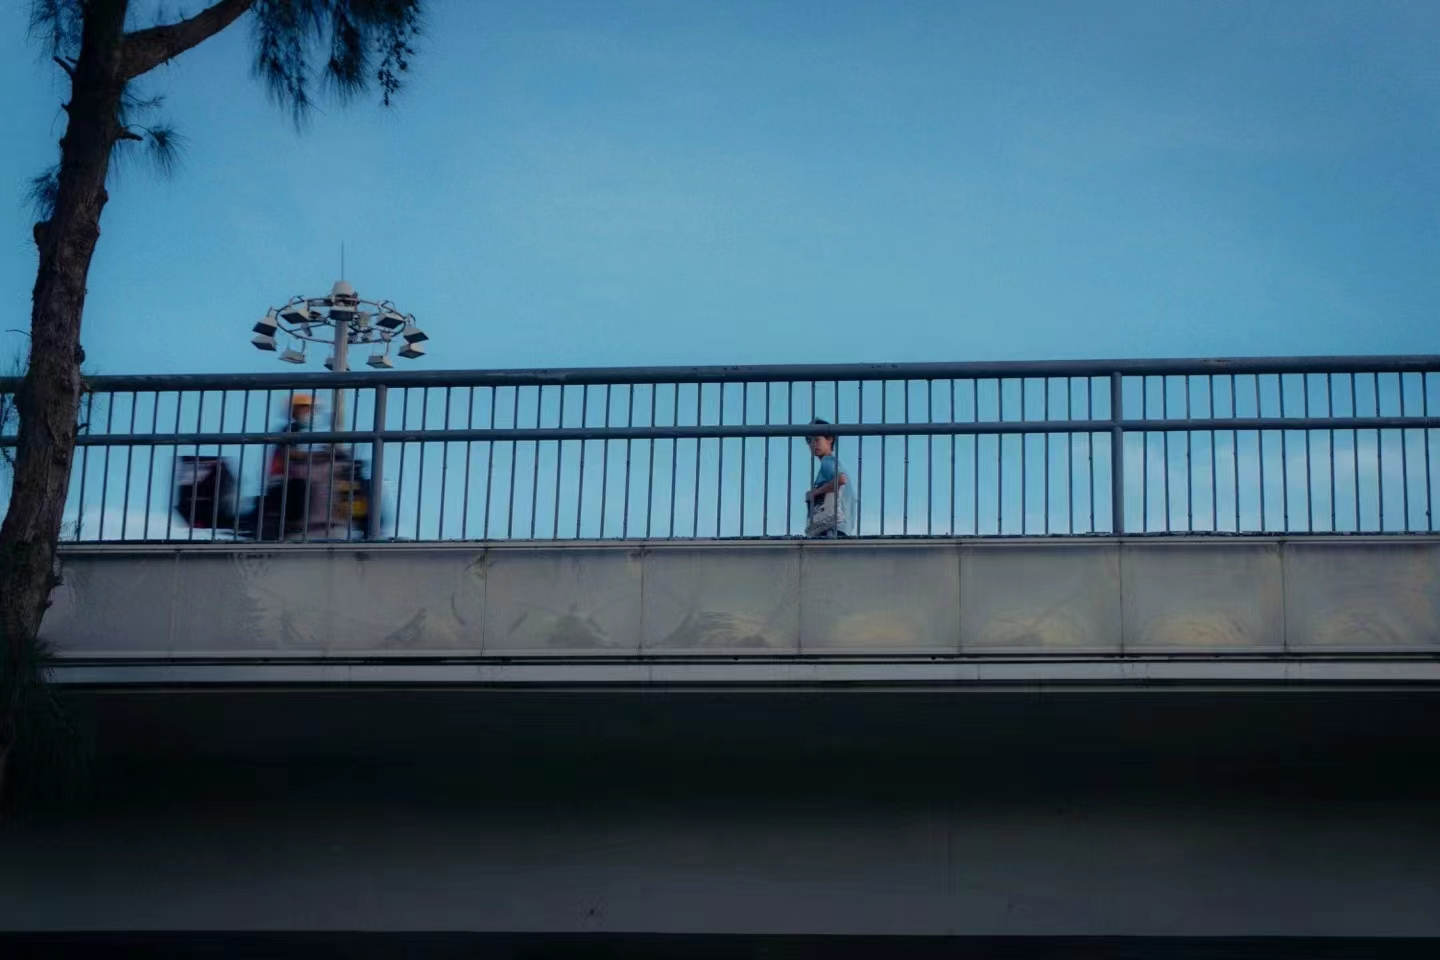
\includegraphics[width=1\linewidth]{example.jpeg}
    \caption{Example}
    \label{fig:example}
\end{figure}
\begin{response}

    \lipsum[6]
\end{response}

\begin{manuscriptchangeenv}{Outer Title}
    \lipsum[7]
    \begin{manuscriptchangeenv}{Inner Title}
        \lipsum[8]
    \end{manuscriptchangeenv}
\end{manuscriptchangeenv}


\bibliographystyle{alpha}
\bibliography{ref}
\end{document}
